\documentclass[conference]{IEEEtran}
\IEEEoverridecommandlockouts
% The preceding line is only needed to identify funding in the first footnote. If that is unneeded, please comment it out.
\usepackage{float}
\usepackage{cite}
\usepackage{amsmath,amssymb,amsfonts}
\usepackage{algorithmic}
\usepackage{graphicx}
\usepackage{textcomp}
\def\BibTeX{{\rm B\kern-.05em{\sc i\kern-.025em b}\kern-.08em
    T\kern-.1667em\lower.7ex\hbox{E}\kern-.125emX}}
\begin{document}

\title{CS 289A Final Project Proposal\\
Driving motion prediction using machine learning
}
\author{
\IEEEauthorblockN{Hengbo Ma}
\IEEEauthorblockA{\textit{SID : 3033121067} \\
hengbo\_ma@berkeley.edu}
\and
\IEEEauthorblockN{Jessica Leu}
\IEEEauthorblockA{\textit{SID : 3033088125} \\
jess.leu24@berkeley.edu}
\and
\IEEEauthorblockN{Franklin Zhao}
\IEEEauthorblockA{\textit{SID : 3033030808} \\
qingan\_zhao@berkeley.edu}
\and
\IEEEauthorblockN{Yujun Zou}
\IEEEauthorblockA{\textit{SID : 27004846} 
\\
yujun\_zou@berkeley.edu}
}

\maketitle


\section{Idea}
As the research field of autonomous driving gets more and more vibrant, motion prediction of the surrounding vehicle also arises as one of the hardest problem that need to be solved, especially at the intersection and roundabout.Many attempts have been made, people tried to classify drivers' type, intention and maneuver. Knowing the fact that many control engineers actually do motion planing by solving an optimization problem, we come up with an idea that we can model all the cars' motion, both human driving car and autonomous driving car, as the optimal trajectory generated by solving an optimization problem (i.e. driving policy of the car). By using this optimal policy in the simulation scenario as baseline, with some existing trajectory analysis dataset such as NGSIM \cite{b1} and KITTI \cite{b2}, we intend to learn the human and robot driving behavior models. The proposed method is done through the following steps. First, define parameter range for several different types of driver and generate optimal trajectory as the training data. Second, learn the driving policy of a new car based on the training data and give the behavior model. Finally, predict the future trajectory of the new car based on the behavior model.

\section{Problem Description}
Among all the setting in autonomous driving scenes, one of the most complicated one is at an intersection with only stop signs and no traffic light. A scenario is shown in Fig.1, where the car on the left (target car) suddenly encounters a car coming from its left in a high speed and doesn't seem to stop. In the simplest case, the target car will have two choices, one is to stop immediately and let the crazy car go first, another choice is to continue moving forward but deviates a bit to avoid collision. The decision made by the target car will influence the decision making of the ego car. If the target car decides to stop, the ego car can go straight, while in the other case the ego car should better stop. Therefore, the ego car's prediction of the target car becomes important.
\begin{figure}[h!]
\centering
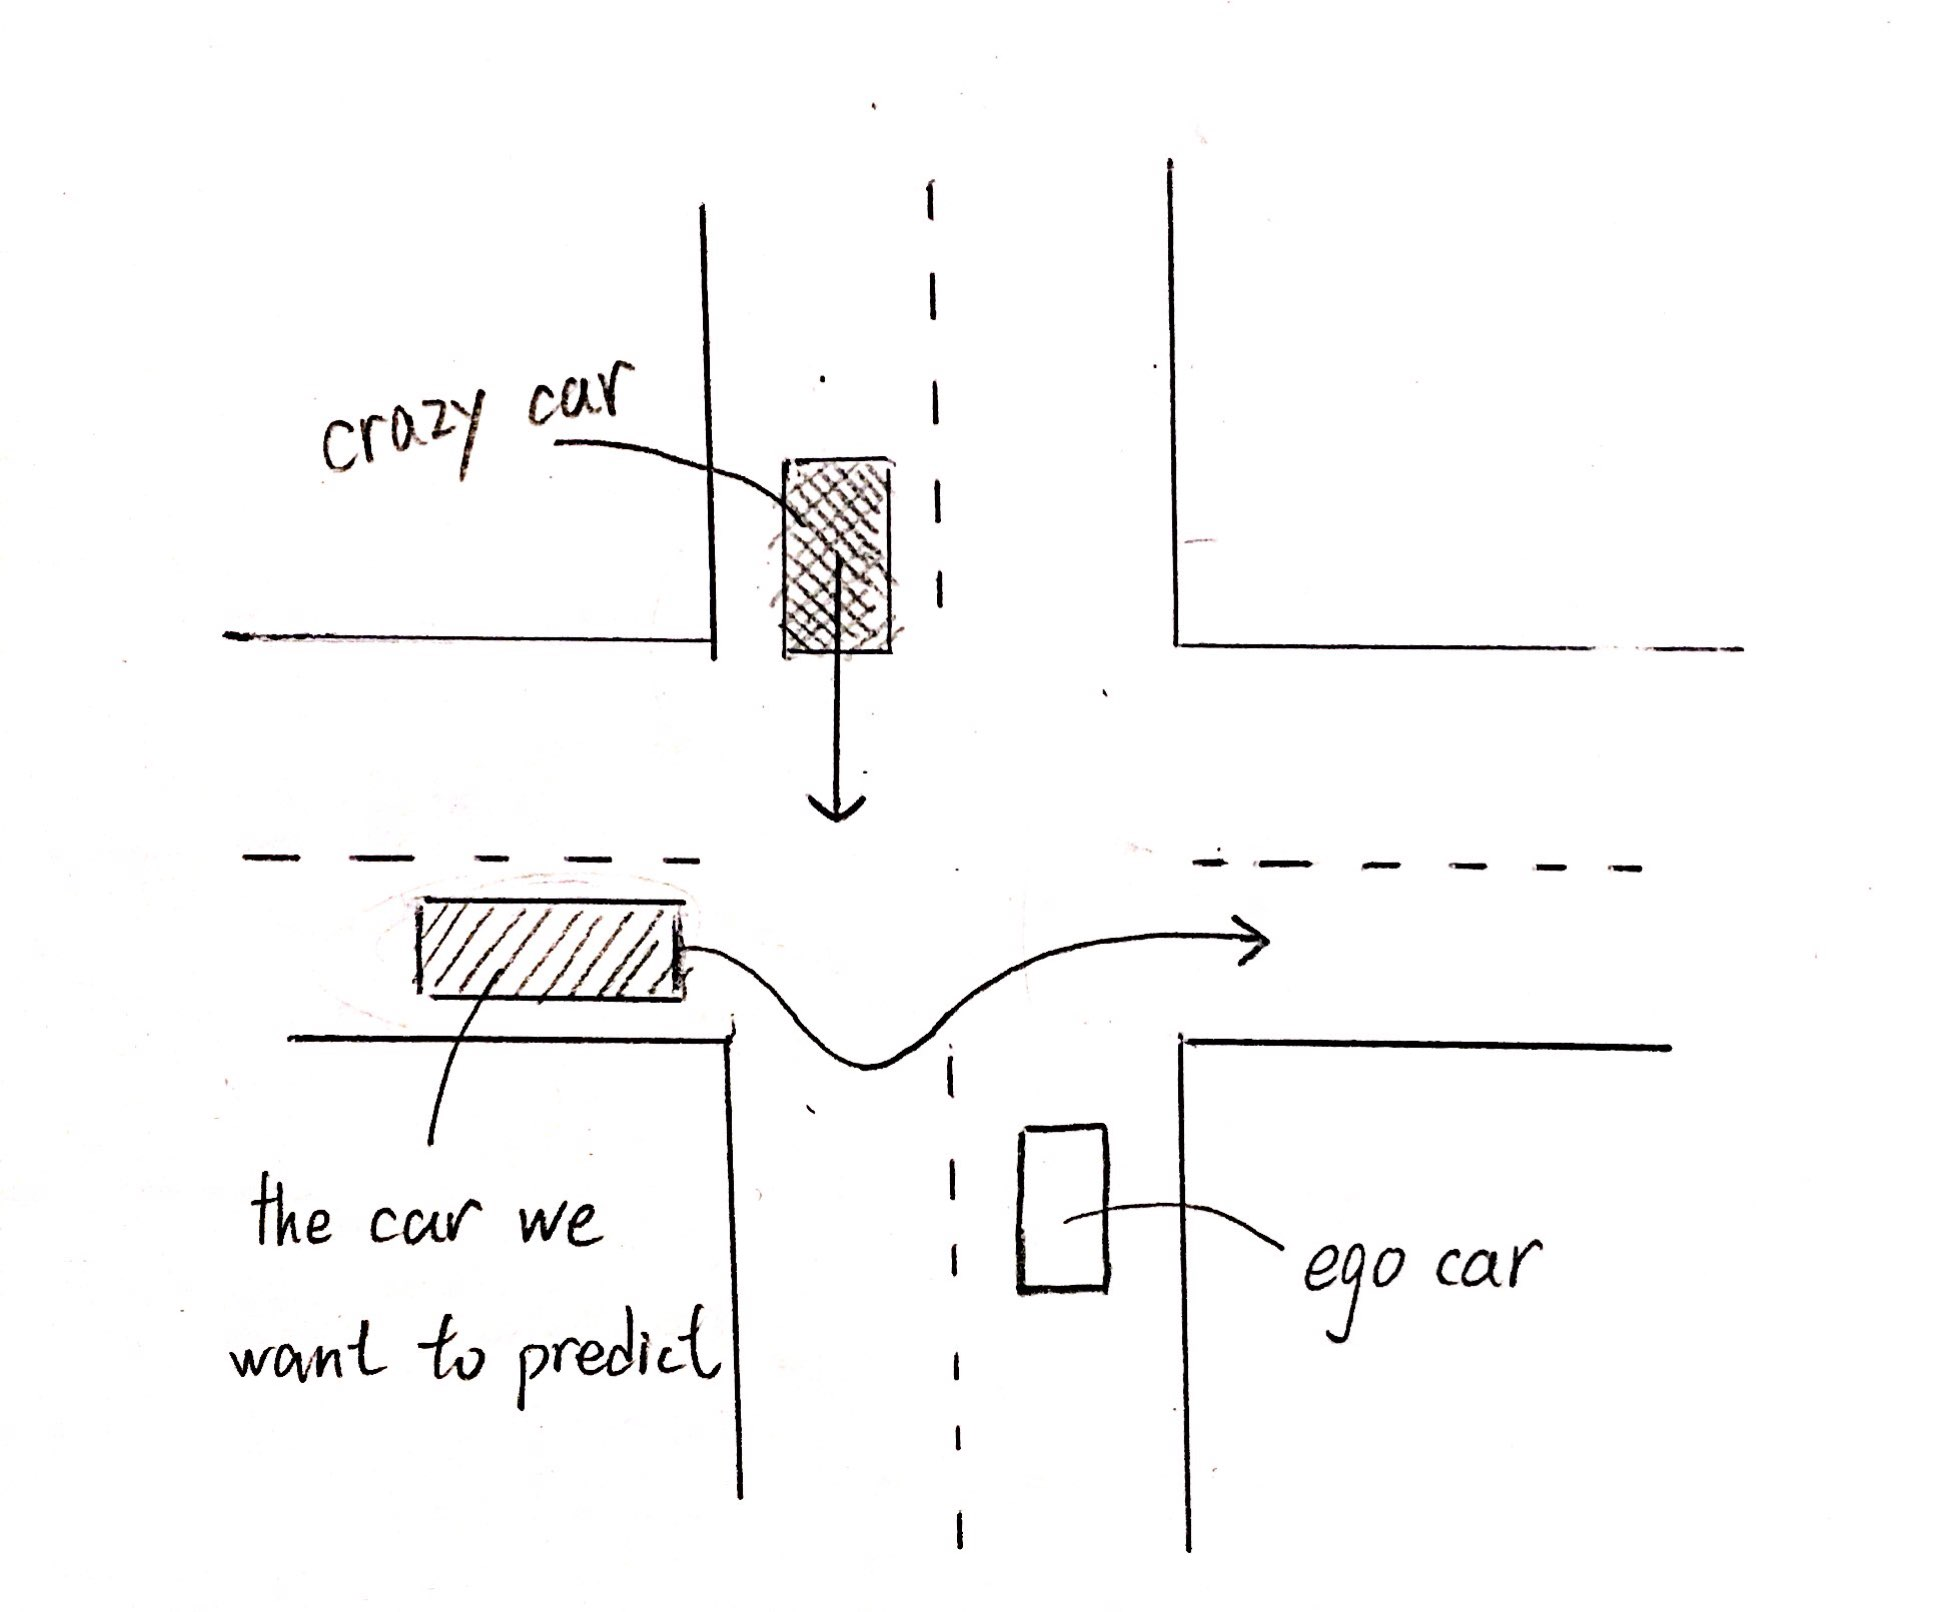
\includegraphics[scale = 0.08]{problem.png}
\caption{Illustration of the setting for our project}
\label{fig:reftraj}
\end{figure}

\section{Methods}

\subsection{Data generation}

According to general driving rules in the U.S., we can roughly classify drivers into three types, constrictive, neutral, and aggressive. The training data is generated by doing simulation of motion planning. The motion planning is done by a control frame work called Model Predictive Control (MPC). The idea of this MPC frame work is to solve an optimization problem that outputs the optimal trajectory for some number of future step. In this work, we set the parameters and construct the optimization problem according to the label, the driver's type, and run the simulation to generate the corresponding output trajectory. As the same time, we will blend some trajectories from the NGSIM \cite{b1} and KITTI \cite{b2} datasets.

\subsection{Learning behavior}

Since the human driving behavior is very complicated and intractable, a subtle model needs to be proposed to describe the structure of human driving behavior. We propose to utilize the probabilistic graph model like Hidden Markov Model to inference the posterior probability given limited observations of current and historical states. We would like to use recurrent neural network such as LSTM to model the probabilistic distribution. 

\subsection{Prediction}

When we have the behavior model, we will use this model to predict the short term and long term trajectory of target car. We hope to get a distribution of the future motion. This will be helpful to make decision and motion planning.


\begin{thebibliography}{00}
\bibitem{b1}US Department of Transportation, “NGSIM – Next Generation Simulation,”, 2007,
http://www.ngsim.fhwa.dot.gov – Access date: May 5, 2007.

\bibitem{b2}Andreas Geiger and Philip Lenz and Christoph Stiller and Raquel Urtasun, Vision meets Robotics: The KITTI Dataset, International Journal of Robotics Research (IJRR), 2013.


\end{thebibliography}

\end{document}
